\documentclass[12pt, a4paper]{article}

\usepackage[utf8]{inputenc}
% Limit the page margin to only 1 inch.
\usepackage[margin=1in]{geometry}

%Imports biblatex package
\usepackage[
backend=biber,
style=alphabetic
]{biblatex}
\addbibresource{../../algs4e.bib}

% Enables the `align' environment.
\usepackage{amsmath}
% Provides useful environments, such as:
% - \begin{proof} ...\end{proof}
\usepackage{amsthm}
\usepackage[most]{tcolorbox}

\newtheorem*{proposition}{Proposition}

% Enables using \mathbb{}, for example \mathbb{N} for the set of natural numbers.
\usepackage{amssymb}

% Allows using letters in enumerate list environment. Use, for example:
%\begin{enumerate}[label=(\alph*)]
% ...
%\end{enumerate}
\usepackage[inline]{enumitem}

% Enable importing external graphic files and provides useful commannds, like \graphicspath{}
\usepackage{graphicx}
% Images are located in a directory called images in the current directory.
\graphicspath{{./images/}}

% Make links look better by default.
% See: https://tex.stackexchange.com/questions/823/remove-ugly-borders-around-clickable-cross-references-and-hyperlinks
\usepackage[hidelinks]{hyperref}
\usepackage{xcolor}
\hypersetup{
	colorlinks,
	linkcolor={red!50!black},
	citecolor={blue!50!black},
	urlcolor={blue!80!black}
}


% Code Listings. Source:
% https://stackoverflow.com/questions/3175105/inserting-code-in-this-latex-document-with-indentation
\usepackage{listings}
\usepackage{color}

\definecolor{dkgreen}{rgb}{0,0.6,0}
\definecolor{gray}{rgb}{0.5,0.5,0.5}
\definecolor{mauve}{rgb}{0.58,0,0.82}

\lstset{frame=tb,
	language=Java,
	aboveskip=3mm,
	belowskip=3mm,
	showstringspaces=false,
	columns=flexible,
	basicstyle={\small\ttfamily},
	numbers=none,
	numberstyle=\tiny\color{gray},
	keywordstyle=\color{blue},
	commentstyle=\color{dkgreen},
	stringstyle=\color{mauve},
	breaklines=true,
	breakatwhitespace=true,
	tabsize=3
}

\newcommand{\prob}{\text{P}}
%\newcommand{\complement}{\mathsf{c}}

% Define an environment called "ex" (for Exercise) so that I can do: \begin{ex}{1.5}...\end{ex}
\newenvironment{ex}[2][Exercise]
{\par\medskip\noindent \textbf{#1 #2.}}
{\medskip}

% Define a solution environment, similar to ex (exercise) environment.
\newenvironment{sol}[1][Solution]
{\par\medskip\noindent \textbf{#1.} }
{\medskip}

\begin{document}
	\noindent Sergio E. Garcia Tapia \hfill
	
	\noindent \emph{Algorithms} by Sedgewick and Wayne (4th edition) \cite{sedgewick_wayne}\hfill
	
	\noindent January 25, 2025\hfill 
	\section*{5.2: Tries}
	\begin{ex}{1}
		Draw the $R$-way trie that results when the keys
		\begin{lstlisting}[language={}]
			no is th ti fo al go pe to co to th ai of th pa
		\end{lstlisting}
		are inserted in that order into an initially empty trie (do not draw null links).
	\end{ex}
	\begin{sol}
		See Figure~\ref{fig:ex-01}.
		\begin{figure}
			\centering
			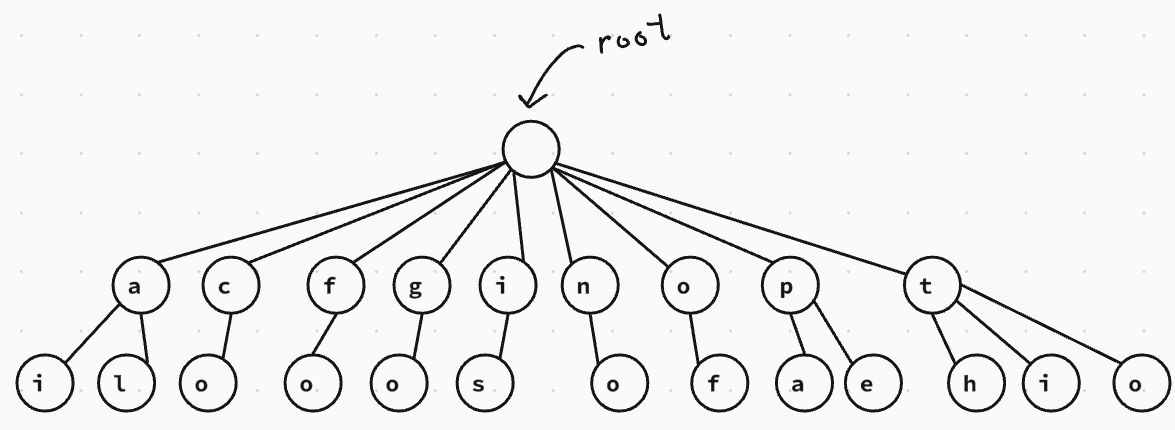
\includegraphics[width=0.8\textwidth]{exercise-01}
			\caption{R-way trie for Exercise 1.}
			\label{fig:ex-01}.
		\end{figure}
	\end{sol}
	\begin{ex}{2}
		Draw the TST that results when the keys
		\begin{lstlisting}[language={}]
			no is th ti fo al go pe to co to th ai of th pa
		\end{lstlisting}
		are inserted in that order into an initially empty TST.
	\end{ex}
	\begin{sol}
		See Figure~\ref{fig:ex-02}.
		\begin{figure}
			\centering
			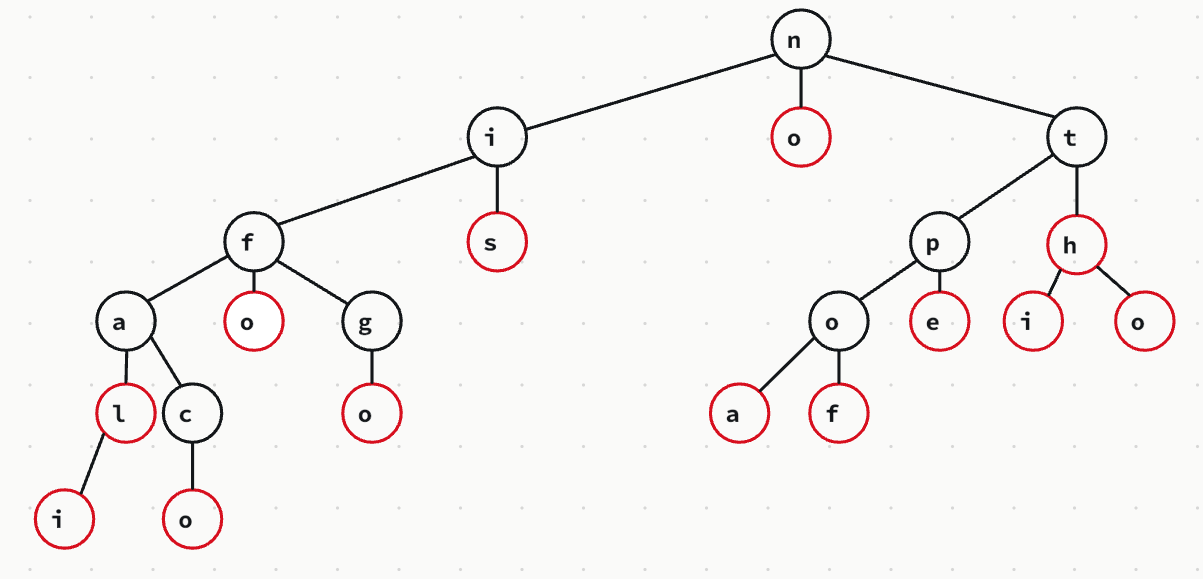
\includegraphics[width=0.6\textwidth]{exercise-02}
			\caption{TST for Exercise 2.}
			\label{fig:ex-02}.
		\end{figure}
	\end{sol}
	\begin{ex}{3}
		Draw the $R$-way trie that results when the keys
		\begin{lstlisting}[language={}]
			now is the time for all good people to come to the aid of
		\end{lstlisting}
		are inserted in that order into an initially empty trie (do not draw null links).
	\end{ex}
	\begin{sol}
		See Figure~\ref{fig:ex-03}.
		\begin{figure}
		\centering
		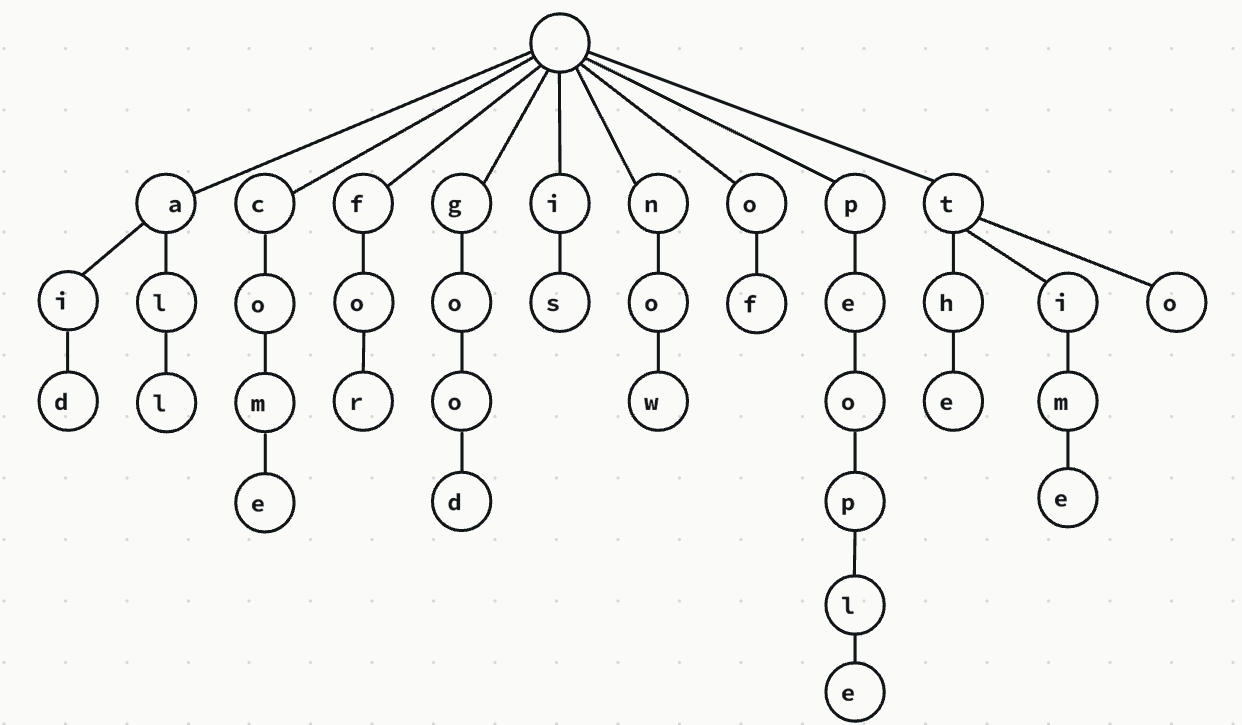
\includegraphics[width=0.6\textwidth]{exercise-03}
		\caption{$R$-way trie for Exercise 3.}
		\label{fig:ex-03}.
		\end{figure}
	\end{sol}
	\begin{ex}{4}
		Draw the TST that results when the keys
		\begin{lstlisting}[language={}]
			now is the time for all good people to come to the aid of
		\end{lstlisting}
		are inserted in that order into an initially empty TST.
	\end{ex}
	\begin{sol}
		See Figure~\ref{fig:ex-04}.
		\begin{figure}
			\centering
			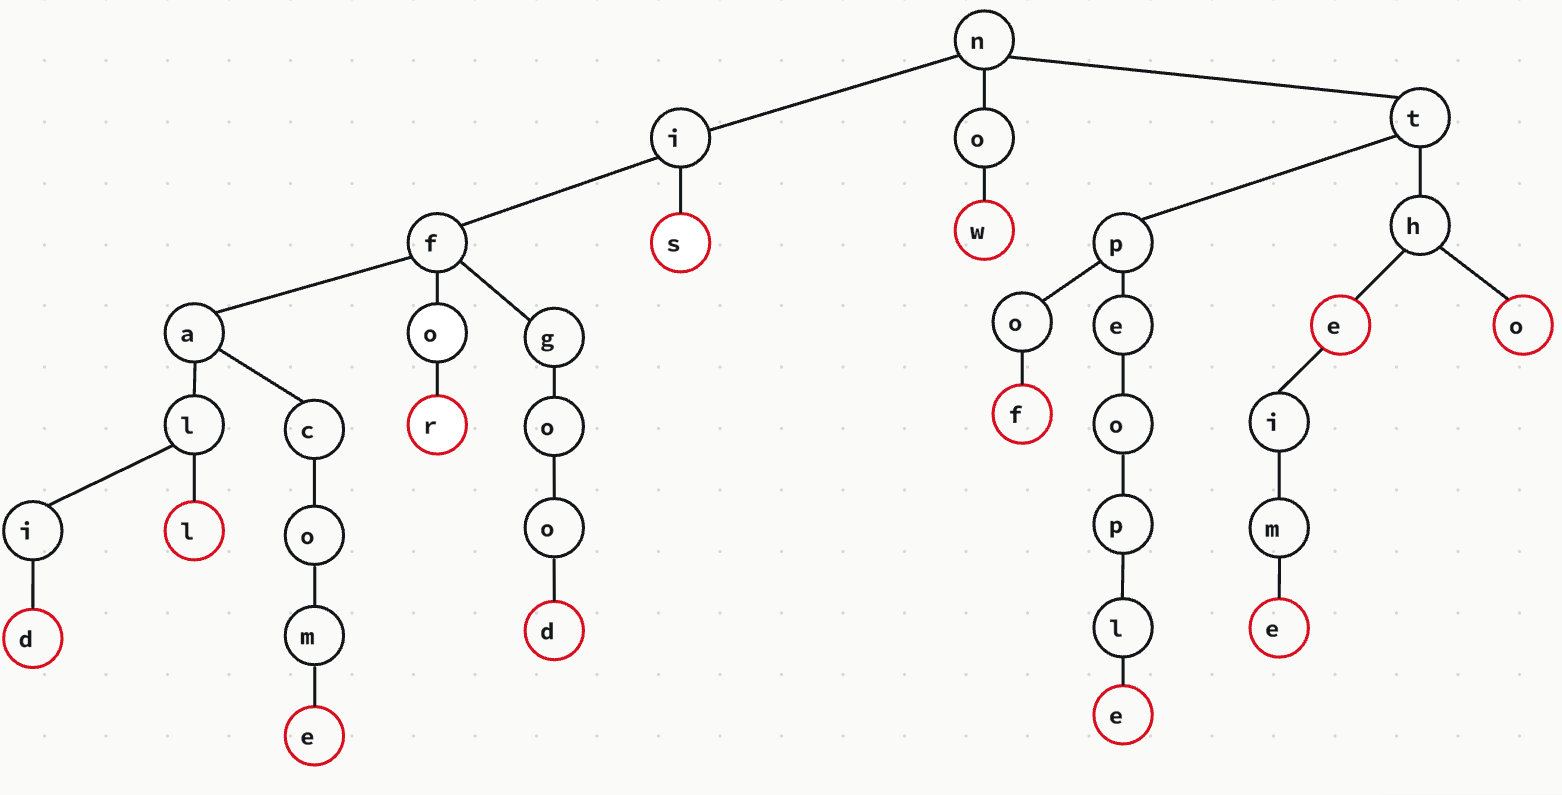
\includegraphics[width=0.6\textwidth]{exercise-04}
			\caption{TST for Exercise 4.}
			\label{fig:ex-04}.
		\end{figure}
	\end{sol}
	\begin{ex}{5}
		Develop nonrecursive versions of \texttt{TrieST} and \texttt{TST}.
	\end{ex}
	\begin{sol}
		See \texttt{com.segarciat.algs4.ch5.sec2.ex05}.
	\end{sol}
	\begin{ex}{6}
		Implement the following API, for a \texttt{StringSET} data type:
		\begin{lstlisting}[language={}]
                StringSET            // create a string set
          void add(String key)       // put key into the set
          void delete(String key)  // remove key from the set
       boolean contains()            // is key in the set?
       boolean isEmpty()         // is the set empty?
            int size()           // number of keys in the set
         String toString()       // string representation of the set
		\end{lstlisting}
	\end{ex}
	\begin{sol}
		See \texttt{com.segarciat.algs4.ch5.sec2.ex06}.
	\end{sol}
	\begin{ex}{10}
		\emph{Size}: Implement very eager \texttt{size()} (that keeps in each node the
		number of keys in its subtree) for \texttt{TrieST} and \texttt{TST}.
	\end{ex}
	\begin{sol}
		See \texttt{com.segarciat.algs4.ch5.sec.ex05}, my non-recursive implementations
		of these classes. There, I provided a very eager implementation of \texttt{size()}.
	\end{sol}
	\pagebreak
	\printbibliography
\end{document}